\documentclass[swedish]{maucsthesis}
%\documentclass[english]{maucsthesis}
% Choose if you write in Swedish or English. (Don't write in English!)
\usepackage{natbib}
\bibliographystyle{agsm}

%
% Select character encoding
%\usepackage[utf8]{inputenc} % depends on system character encoding, most Linux use utf8, your mileage may vary!
\usepackage[T1]{fontenc} % Use this character encoding with Overleaf (www.overleaf.com)!

\usepackage{graphicx}
\graphicspath{ {./bilder/} }

\usepackage{titlesec}
\newcommand{\sectionbreak}{\clearpage}

\usepackage{float}

\usepackage{csquotes}

\begin{document}

\swedishtitle{Rättsäker Textanalys}
\englishtitle{Title in English}

\author{Kalle Lindqvist \and Henrik Svensson}

\level{grundnivå}
\credits{15}
\degree{kandidatexamen 180 hp}
\subject{datavetenskap}
\studyprogram{informationsarkitektur}

\seminardate{2019-04-24}

\supervisor{Johan Holmberg}
\examiner{Vicke Viking}
\maketitle % This constructs MaU title page from info above

\begin{sammanfattning}
  Språkteknologi är ett forskningsområde där det ständigt görs nya framsteg. En
  betydande del av den textanalys som sker inom detta fält har målet att uppnå
  en fullgod tillämpning kring dialogen mellan människa och dator. I denna
  studie vill vi istället fokusera på vilken inverkan språkteknologi kan ha på
  den mänskliga inlärningsprocessen. Vårt praktiska testområde har samtidigt en
  framtida inverkan för en av de mest grundläggande förutsättningarna för ett
  rättssäkert samhälle, nämligen den polisiära rapportskrivningen.

  Genom att skapa en teoretisk idébas som förenar viktiga aspekter av både
  språkteknologi liksom officiell polisrapportskrivning och därefter
  implementera den i en pedagogisk webbplattform ämnad för polisstudenter är vi
  av uppfattningen att vår forskning tillför något nytt inom det
  datavetenskapliga respektive sociologiska fälten.

  Syftet med arbetet är att verka som de första stegen mot en webbapplikation
  som understödjer svensk polisdokumentationen.
\end{sammanfattning}

\begin{abstract}
Text in English\ldots
\end{abstract}

% This is sort of magic, do not touch
\ifodd\value{page}\else\mbox{}\newpage\fi
\tableofcontents
\newpage
\startpagecount

\section{Inledning}

\subsection{Forskningsmål}

Syftet med projektet är att undersöka om en applikation för textanalys kan
hjälpa studenter på svenska polisutbildningar att skapa mer rättssäkra
polisrapporter. Studenter ska kunna ladda upp sina rapporter i den webbaserade
applikationen där sedan stavningskontroll samt grammatiska, språkliga och
tonalitetsanalyser genomförs. Applikationen ska även kontrollera att rapporten
är skriven i enlighet med den svenska polismyndighetens riktlinjer så att den
uppfyller rättssäkerhetsaspekten. Efter det att denna analys har gjorts ska
feedback skickas till studenterna om de fel och brister som bör åtgärdas innan
polisrapporten kan vidarebefordras till en lärare.

\subsubsection{Forskningsfrågor}

\begin{itemize}
\item Hur kan polisstudenters rapporter bli mer rättssäkra genom digital
  textanalys?
\item Hur kan rättningsarbetet för lärare vid polisutbildningarna bli mer
  effektivt med hjälp av digital textanalys?
\end{itemize}

\subsection{Avgränsning}

Vid en intervju som ägde rum den 31 januari 2019 med Per Esbjörnsson rangordnade
han kraven på applikationen enligt följande:

\begin{enumerate}
\item Applikationen ska kontrollera att rubrikerna är korrekta
\item En semantisk analys ska göras som kontrollerar att den nödvändig
  informationen finns med under rubrikerna.
\item Grammatiska, lingvistiska och rättstavningskontroller ska genomföras
\item En tonalitetsanalys ska göras
\item Information ska skickas till läraren om inlämningen    
\end{enumerate}
Det sista kravet är baserat på Per Esbjörnssons önskan om att då rapporten når
läraren så ska denne också erhålla information om eventuella fel som noterades
och hur många gånger rapporten analyserades. Vi har emellertid beslutat att
detta kommer ligga utanför projektets omfattning på grund av den korta tiden vi
har tilldelats för att utveckling av applikationen, strax över 11 veckor, och
dess placering i kravlistan. Under mötet uttryckte Per Esbjörnsson också en
önskan att applikationen ska kunna integreras i Canvas, vilket är den
läroplattform som används av studenter och lärare vid polisutbildningen i Malmö.
Även detta kommer att ligga utanför projektets omfattning på grund av att
utbildningen i Malmö förväntas ändra läroplattform från Canvas till ett internt
system i början av nästa termin. Vårt mål är emellertid att applikationen ska
vara så oberoende att en integration är möjlig i det nya systemet.

\subsection{Bakgrund}
I december 2017 meddelade den svenska regeringen att 10 000 nya poliser skulle
utbildas inom en sjuårsperiod. En ny polisutbildning skulle upprättas i Malmö
som ett initiativ för att uppnå detta mål, och skulle komma att bli Sveriges
fjärde polisutbildning efter de som finns vid lärosätena i Umeå, Växjö och
Stockholm. Den nya polisutbildningen med 96 registrerade studenter öppnade vid
Malmö Universitetet i samband med vårterminens start i början av 2019.

I enlighet med deras utbildningsplan studerar eleverna bland annat ämnen som
juridik, kriminologi, beteendevetenskap, brottsutredning, förhör och
intervjuteknik. Enligt Per Esbjörnsson, lärare vid polisutbildningen, blev det
redan under den första kursen, Grunder i polisiärt arbete, uppenbart att de
främsta problemen som studenterna tampades med var att skriva polisrapporter på
ett korrekt och rättssäkert sätt. Problemen inkluderade att skriva korrekta
rubriker i enlighet med klassificering, grammatisk, att hålla passande
tonaliteten samt att undvika nedsättande termer i rapporterna. För lärarna vid
polisutbildningen i Malmö blev rättningsprocessen av polisrapporterna en
tidskrävande uppgift som stal tid från annan viktig utbildning.

\subsection{Relaterad forskning}

Det finns två särskilda studier som har ägt rum inom dessa områden under det
senaste decenniet och som är av intresse för oss.

I en studie som genomfördes vid Zürichs universitet gjordes ett försök att
implementera lingvistiskt redigeringsstöd för att underlätta skrivprocessen för
skribenter. I den vetenskapliga undersökningen som ledde fram till processen
fann \cite{Piotrowski:2009} att mycket lite forskning fanns tillgänglig om att
stödja skapandet av textinnehåll. I det som \citeauthor{Piotrowski:2009} kom att
kalla LingURed-projektet utvecklade de en uppsättning språkmedvetna
redigeringsverktyg som kunde analysera teckensträngar utifrån dess språkliga
struktur. Även om dessa verktyg inte skulle kunna ge lingvistisk vägledning åt
författarna så hjälpte de dem att skapa meningar med färre fel.

\cite{zhu:2015} har noterat att sedan dess har antalet korpusar, som är stora
samlingar av texter som kan analyseras automatiskt för lingvistiska mönster och
strukturer, ökat. De flesta korpus är dock avsedda för lingvistisk forskning och
inte för utbildning. Med detta i åtanke byggde \citeauthor{zhu:2015} ett
digitalt korpusverktyg som kallades Text X-Ray som skulle hjälpa både lärare och
studenter att analysera sin egna skrivkorpusar och att jämföra dem med andra.
Under våren 2013 genomfördes en studie med flera engelskspråkiga lärare på
högskolor över hela världen för att avgöra om Text X-Ray skulle ha en inverkan
vid riktiga utbildningstillfällen. Funktionerna som verktyget erbjöd var bland
annat att belysa grammatiska fel för att öka elevernas förmåga att rätta problem
som hällde grundläggande meningsstruktur. Text X-Ray mätte även och visade
komplexiteten i en skriftlig mening sett till dess längd.

\subsection{Språkteknologi}

Då lingvistik definieras som studien av mänskliga språk kan datalingvistik ses
som teorierna och modellerna av detta område i en maskinell representation. Det
grundläggande syftet med datalingvistik är att konstruera modeller av
språkstrukturer så att automatiseringen av språkbehandling exempelvis kan göras
digitalt. Språkteknologi och datalingvistik är båda fält som ständigt utforskas
av IT-industrin och som når nya resultat. Idealiskt, och kanske inom en snar
framtid, ska exempelvis datorer kunna analysera stora mängder text, parsa
skriftliga meningar och utföra morfologisk redigering till perfektion med hjälp
av digital språkbehandling \citep{nugues:2014}.

Idag finns det olika verktyg som kan utföra automatiska analyser av språkliga
attribut i texter. Dessa program, som innehåller så kallad "lingvistisk kunskap"
i form av vokabulärer av grammatiska strukturer, är baserad på det
tvärvetenskapliga forskningsområdet språkteknologi. Det finns många lingvistiska
resurser som språkteknologi täcker, inte minst en mängd lexikon, ordböcker,
termbanker, databaser, ordböcker samt olika digitala verktyg för att analysera
språk. Dessa verktyg är oftast utrustade med funktionaliteter som stavnings- och
grammatiska analyseringsverktyg samt så kallade läsbarhetsindexar (LIX)
*hänvsining till annat avsnitt* för att beräkna hur många och vilka grammatiska
fel som är vanligt förekommande i en skriftlig text. Sådana program har kunnat
spara tid i rättningsprocesser \citep{wengelin:2017}.

\subsection{Rapportskrivning}

Den svenska polisförordningen stipulerar att poliser ska uppträda på ett sätt
som skapar tilltro hos allmänheten. Att ha en korrekt språklig kommunikation,
något som bland annat sker genom skriftliga rapporter, är en viktig aspekt av
den polisiära yrkesutövningen. Inte minst med tanke på att det finns många
potentiella läsare av en polisrapport – jurister i form av åklagare och
försvarsadvokater, brottsoffer och förövare, journalister och personer ur
allmänheten. Polisrapporter utgör också ofta grunden för juridiska ärenden. En
övertygande beskrivning av en händelse kan till exempel vara avgörande för om en
åklagare väljer att väcka åtal eller inte. Därför är det särskilt viktigt att
polisrapporter skrivs på ett begripligt och korrekt sätt \cite{ask:2013}.
Ordvalen i rapporterna är också av särskild vikt då poliser bör använda ett
språk som är objektivt, detta för att rapporten ska kunna uppnå rättssäkerhet
\citep{ask:2018}. En viktig aspekt för att uppnå det är att ett etiskt
förhållningssätt präglar texten. Bland annat förutsätts det att nedsättande
formuleringar inte bör förekomma i polisrapporter, annat än om dessa är tydligt
citerades från ett vittne. I sådana fall bör de nedsättande termerna omgärdas av
citattecken \cite{ask:2013}.

Durtvå är namnet på det svenska polisens interna IT-system där all dokumentation
upprättas digitalt. Polismyndigheten har fastställt ett antal riktlinjer för
denna dokumentation, bland dem rekommenderas att poliserna använder sig av vissa
standardrubriker. Enligt Per Esbjörnsson utgör dessa rekommendationer också
grunden för hur polisstuderande instrueras att utforma sina rapporter. De
vanligaste rekommenderade rubrikerna för polisrapporterna är följande:

\begin{itemize}
\item Brottet - här beskrivs brottet kortfattat, förfarande, skador, rekvisita
  och, om möjligt, avsikt
\item Skador - gäller både egendom och person och hur de inträffade
\item Signalement
\item Ersättningskrav
\item Övrigt - annan eventuell information som kan vara användbar
\end{itemize}

I fall då ett brott inte misstänks ha begåtts ska den första rubriken ersättas
av Händelsen, följt av rubriken Händelseförloppet. Det finns också två
rekommenderade rubriker för att inkludera vid behov. Dessa är Vittnen och
Brottsplatsundersökning. Riktlinjerna för Durtvå är dock inte den enda interna
dokumentationen för rapportskrivning som finns tillgängligt för polisstudenter.
Lärare på polisutbildningen vid Linnéuniversitetet i Växjö har sammanställt ett
dokument där de listar 15 tips för att skriva en bra polisrapport. Detta
dokument, som också används i utbildningen i Malmö, innehåller tips som
inkluderar att rubriker måste skrivas i versaler, att texten ska vara lätt att
förstå, att samma tempus ska vara genomgående i rapporten och att förkortningar
i bör användas. Därtill att en så korrekt brottsplatsadress som möjligt bör
anges liksom korrekt anmälningstid och brottstid.

\section{Metod}

\subsection{Ramverk}

När forskning bedrivs som är baserad på informationssystem liknande det vi
utvecklar och utvärderar i detta projekt rekommenderar \cite{hevner:2004} att
processen bäst görs via konceptuella ramverk som positionerar och jämför
beteendevetenskapliga och designvetenskapliga paradigmer med varandra. En sådan
process underbygger förståelsen, genomförandet och utvärderingen av
informationssystemforskning. Nedan presenteras en representation av the
Information Systems Research Framework som tagits fram av
\citeauthor{hevner:2004}.

\begin{figure}[H]
    \centering
    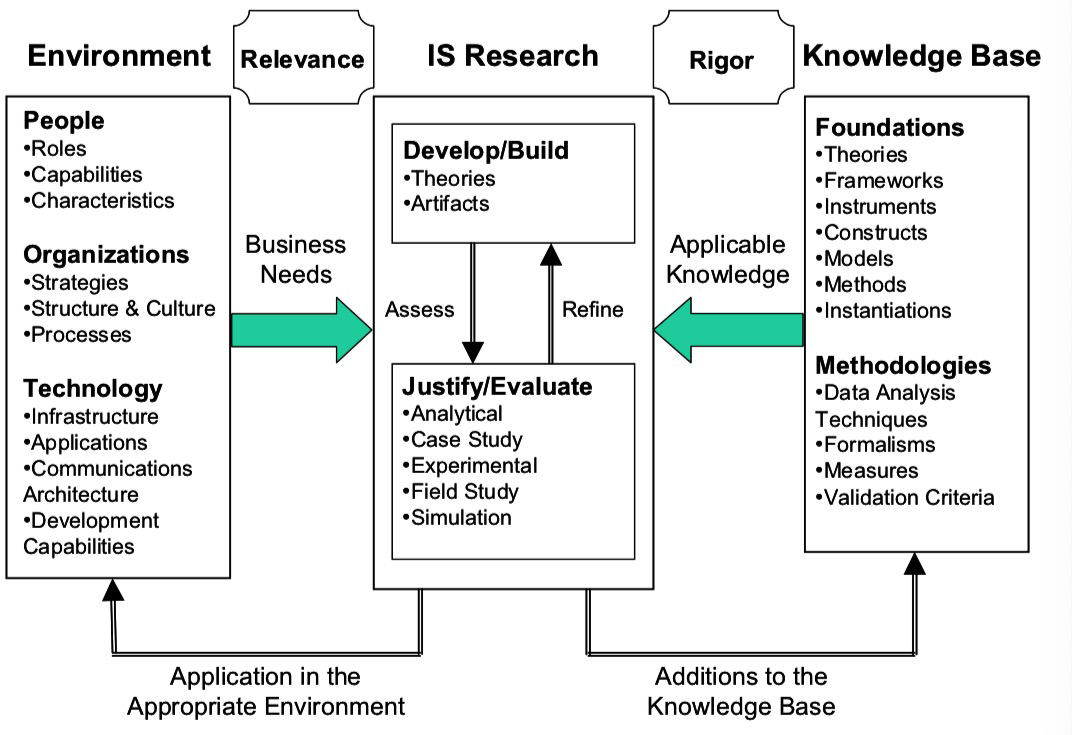
\includegraphics[width=0.75\textwidth]{isframework}
    \caption{Översikt av Information Systems Research Framework}
    \label{fig:isframework}
\end{figure}

Problemen som uppfattas av forskaren definieras i arbetsmiljön. Detta fält
består av personer, organisationer och den befintliga eller planerade teknologin
hos dem. Affärsbehoven skapas utifrån dessa tre faktorer. Organisationen
kännetecknas av strategi, struktur och kultur samt befintliga affärsprocesser.
På samma sätt formas de av rollerna, egenskaperna och kännetecknen hos
personerna i organisationen. Slutligen bidrar den nuvarande tekniska
infrastrukturen, applikationerna, kommunikationsarkitekturer och
utvecklingsmöjligheter till att definiera dem.

Personer i detta projektets arbetsmiljö utgörs således av polisstudenter liksom
lärare. Studenterna har behov av hjälpmedel i utformningen av polisrapporter på
ett rättssäkert sätt, medan lärarna å sin sida behöver få hjälp med
rättningsprocessen av dessa. Båda rollerna kännetecknas av ett mindre tekniskt
kunnande och intresse, vilket skapar behovet av ett användarvänlig system.

Organisationen som de ingår i är polisutbildningen vid Malmö universitet vars
strategi bland annat är att utbilda studenter till färdiga polisaspiranter med
kunskap att skriva polisrapporter på korrekt sätt. Den teknologi som finns till
förfogande är för tillfället läroplattformen Canvas där rapporterna lämnas in
och omdömen om dessa ges. Allt eftersom affärsbehoven definieras genomförs är
forskningen i två faser som är integrerade med varandra. De
beteendevetenskapliga paradigmerna behandlar forskning genom utveckling och
rättfärdigande av teorierna. Samma teorier som hjälper till att förklara eller
förutsäga fenomen i förhållande till affärsbehoven.

Vår teori är att en språkteknologisk applikation som genomför automatisk
textkontroll av en rapport och återkopplar brister i denna med konstruktiv
respons kan möta de aktuella affärsbehoven för detta projekt. Ett av våra
antagande är också att studenter genom de felmeddelanden som applikationen
återger också kan fördjupa sin förståelse av vikten av rättssäkerhet inom ramen
för polisrapporter. Artefakten varpå vi vill rättfärdiga dessa teorier är
applikationen vi byggt, konstruktionen av denna beskrivs i avsnittet Utveckling.

Precis som ramverket rekommenderar en iterativ process i utvecklingen och
utvärderandet av artefakten, så har arbetet i detta projekt kommit att bestå av
fyra stora iterationer:

\begin{enumerate}
\item Den första utgick från vårt initiala möte med Per Esbjörnsson och
  konkretiserades genom den kravinsamling som kom att bli resultatet av denna.
  Utifrån de önskemål och krav på artefakten som beskrevs av Per samt det
  officiella polismaterial som relaterar till hur rapportskrivning ska se ut
  kunde vi sätta upp ramar kring omfattningen av vårt problemområde. I samband
  med mötet fick vi också reda på var och hur artefakten ska integreras och
  kunde därför börja skissa på en tidig design.
\item Den andra iterationen bestod av den litteraturstudie vi gjorde för att
  undersöka existerande forskningen som gjorts inom området, och som finns
  närmare beskrivet i avsnitten Relaterad forskning samt Språkteknologi [ref].
  Utifrån denna studie kunde vi justera våra forskningsmål i enlighet med det
  empiriska material vi fann. Dessa resultaten ledde också till en insikt kring
  hur implementeringen av de olika reglerna för rapportskrivning kunde ske.
\item Den tredje iterationen bestod av en första instansiering av artefakten,
  vilket var i form av en tidig prototyp av webbapplikationen och APIet [bild].
  Under den inledande fasen av iterationen fick vi tillgång till övningsmaterial
  bestående av uppgiftsbeskrivningar och cirka 400 anonymiserade rapporter, där
  80 redan var godkända av lärare och resten hade inte hade rättats. Vi testade
  rapporterna mot vårt textanalysverktyg för att identifiera fel som inte
  beskrivs i den officiella polisdokumentationen, så som felformatteringar och
  inkorrekta filformat, samt eventuella buggar i applikationen. Här kunde de
  godkända rapporterna också hjälpa oss att identifiera de gränsvärden som var
  användbara för vår tonalitetsanalys och läsbarhetsanalys.
\item Resultatet av den fjärde iterationen bestod av en andra och slutgiltig
  instansiering av applikationen. Denna versionen var ett resultat av de
  ändringar som gjortsvid utvärderingen efter användarstudien, vilka beskrivs i
  avsnittet Önskvärda funktionalitet [ref], och beskrivs i sin helhet i
  avsnittet Applikation [ref].
\end{enumerate}

Mindre iterationer förekom i samtliga av de iterationer som beskrivs ovan. Ju
längre in i processens skede vi kom desto mer frekventa blev dessa mindre
iterationer då vi bland annat genom instansieringarna kunde identifiera fler
nödvändiga funktionaliteter. Kunskapsbasen som presenteras i ramverket består av
fundament och metodologier. Sammansatt gör dessa komponenter att forskningen kan
uppnås. Medan fundamentet skapar teorier, ramverk, instrument, konstruktioner,
modeller, metoder och instanser som används under utvecklingsfasen i
forskningsstudien skapar metodologier riktlinjer som används i berättigande- och
utvärderingsfasen. Metoden för denna process som vi ser det är tillämpningen av
språkstrategi i utformningen av polisrapporter medan är instansieringen ett
arbetssystem som visar användningen av metoden, i detta fall den applikation vi
konstruerar. Vidare finner vi våra teorier som är genomgående i fundament och
metodologier i den vetenskapliga litteratur vi tillskansat oss genom
litteraturstudien som beskrivs i nedanstående avsnitt. Under utvecklingen har vi
tillgång till en rad anonymiserade studentrapporter som vi kör genom
applikationen för att finna vanliga fel, detta ser vi som dataanalysteknik som
den definieras i metodologifältet.

Stabilitet för vår forskning skapas genom att tillämpa fundament med metodologi.
Då beteendevetenskap och designvetenskap tillämpas på ett företagets behov
bidrar de också samtidigt till innehållet i kunskapsbasen för vidare framtida
forskning \cite{hevner:2004}.

Det finns andra alternativa metoder som kunde använts för att underbygga vårt
arbetet, men som samtidigt av olika anledningar inte heller framstått lika
passande som Information Systems Research Framework.

En av dem är så kallad action research, en metod som kännetecknas av att den
genomförs under en pågående utbildningssession. Detta är en iterativ metod där
forskaren, i detta fallet en lärare, ständigt utforskar strategier och medvetet
analyserar resultat med avsikt att göra justeringar samtidigt som utbildningen
fortskrider \citep{clement:2004}. Då vårt arbete innefattar faktiska lärare och
sker inom kontexten av en utbildning kan action research i teorin ses som ett
passande alternativ för denna studie. Rent praktiskt inser vi dock att det vore
svårt rent logistiskt och tidsmässigt att samordna en sådan utbildningssession
som samtidigt också hade varit användbar för vår forskning.

\subsection{Litteraturstudie}

I detta avsnittet presenterar vi den litteratur i form av artiklar och böcker
som valts och hur vi hittade dem i förhållande till vårt forskningsmål och
frågor.

\subsubsection{Rekommendationer}

En del litteraturen förvärvades genom rekommendation, till stor del från vår
handledare Johan Holmberg. Dessa var:
\begin{itemize}
\item \textit{Language Processing with Perl and Prolog} av Pierre M. Nugues
\item \textit{Design and Creation} av Ozan Saltuk och Ismail Kosan
\item \textit{Design Science in Information Systems Research} av Hevner, Alan et.al.
\end{itemize}

I en icke-systematisk Google-sökning hittade vi Gothenburg University Computer
Linguistics som är en universitetsbaserad databas. Även om det inte gick att
göra sökningar i deras indexering gav vår systematiska genomgång av
publikationerna oss många värdefulla resultat. Här hittade vi följande artiklar:

\begin{itemize}
\item \textit{‘‘What happened?’’ From talk to text in police interrogations} av
  Tessa C. van Charldorp
\item \textit{‘She had it coming?’: An experimental study of text interpretation
    in a police classroom setting} av Sofia Ask
\item \textit{Huvudansatser för parsningsmetoder: Om programutvecklingens
    förutsättningar i en svensk kontext} av Kenneth Wilhelmsson
\end{itemize}

Under en icke-systematisk sökning i Libsearch, bibliotekskatalogen vid Malmö
universitet, fann vi även följande litteratur:

\begin{itemize}
\item \textit{Skrivande Polis} av Sofia Ask
\item \textit{Text och kontext : perspektiv på textanalys} av Åsa Wengelin et al.
\end{itemize}

\subsubsection{Sökprocess}

Då vi skulle söka igenom de databaser som fanns till vårt förfogande ansåg vi
det nödvändigt att resultaten filtreras utifrån ett antal kriterier. Dessa var
att artiklarna var skrivna på svenska eller engelska och inte publicerats
tidigare än 1990. Artiklarna var också tvungna att ha hänvisas till minst en
artikel eller tidskrift. De nyckelord som vi ansåg vara relevanta för den här
studien var följande: digital text analysis, computational linguistics, natural
language processing och police. Vi delade sedan in sökorden och kombinationer av
dessa i fem söktermer. Att vi enbart valde fem termer berodde på det stora antal
databaser vi hade till vårt förfogande. Söktermerna var följande:

\begin{itemize}
\item S1: ‘\textit{digital text analysis}’
\item S2: ‘\textit{computational linguistics}’
\item S3: ‘\textit{digital text analysis}’ AND ‘\textit{computational
    linguistics}’
\item S4: ‘\textit{digital text analysis}’ AND ‘\textit{computational
    linguistics}’ OR ‘\textit{natural language processing}’
\item S5: ‘\textit{police}’ AND ‘\textit{digital text analysis}’ OR
  ‘\textit{computational linguistics}’ OR ‘\textit{natural language processing}’
\end{itemize}

Sökningarna gjordes också på svenska med sökorden översatta enligt följande:
digital textanalys (digital text analysis), datorlingvistik, datalingvistik
(computational linguistics), språkteknologi (natural language processing) och
polis (police).

\subsubsection{Databaser}

De databaser som valde var ACM Digital Library på grund av att den är den
största databasen inom datavetenskap, IEEE Xplore Digital Library som erbjuder
4,5 miljoner dokument från publikationer inom datavetenskap och andra ämnen,
DIVA som är en databas som samlar publikationer från 47 universitet i Sverige,
Linguistics and Language Behavior Abstracts (LLBA) som samlar internationell
litteraturen inom lingvistik och relaterade discipliner inom lingvistik samt
MUEP som är databasen för akademisk litteratur som skapats av lärare och
studenter vid Malmö universitet, där denna uppsats också publiceras. När vi
valde de artiklar som vi trodde var relevanta började vi med att läsa abstraktet
för att bestämma om de var värda att undersöka vidare.

\begin{table}[H]
\centering
\begin{tabular}{|l|l|l|l|l|}
\hline
Databas & Sökning & Resultat & Lästa abstrakt & Hämtade artiklar \\ \hline
ACM     & S1      & 681      & 16             & 1                \\ \hline
ACM     & S2      & 18059    & 24             & 2                \\ \hline
ACM     & S3      & 61       & 6              & 4                \\ \hline
ACM     & S4      & 45       & 1              & 0                \\ \hline
ACM     & S5      & 0        & 0              & 0                \\ \hline
IEEE    & S1      & 156      & 12             & 2                \\ \hline
IEEE    & S2      & 369      & 18             & 0                \\ \hline
IEEE    & S3      & 1        & 1              & 0                \\ \hline
IEEE    & S4      & 2170     & 14             & 3                \\ \hline
IEEE    & S5      & 2435     & 20             & 0                \\ \hline
DiVA    & S1      & 312      & 16             & 0                \\ \hline
DiVA    & S2      & 2906     & 22             & 2                \\ \hline
DiVA    & S3      & 16       & 3              & 1                \\ \hline
DiVA    & S4      & 29       & 5              & 0                \\ \hline
DiVA    & S5      & 0        & 0              & 0                \\ \hline
MUEP    & S1      & 1245     & 31             & 1                \\ \hline
MUEP    & S2      & 380      & 15             & 1                \\ \hline
MUEP    & S3      & 209      & 11             & 0                \\ \hline
MUEP    & S4      & 531      & 12             & 0                \\ \hline
MUEP    & S5      & 175      & 8              & 1                \\ \hline
LLBA    & S1      & 3190     & 14             & 0                \\ \hline
LLBA    & S2      & 14580    & 16             & 3                \\ \hline
LLBA    & S3      & 492      & 10             & 1                \\ \hline
LLBA    & S4      & 10782    & 13             & 1                \\ \hline
LLBA    & S5      & 24439    & 9              & 0                \\ \hline
\end{tabular}
\caption{Resultaten av våra söktermer i databaserna}
\label{searchtable}
\end{table}

\subsection{Utveckling}

% beskrivning av iterationsfaser

\subsection{Användartester}

Då vi eftersträvar att applikationen ska vara användarvänlig och effektiv bör vi
försöka att generera mätvärden av typen UX (user experience) som kan säkerställa
att applikationen når upp till dessa egenskaper. UX-mätvärden är baserade på ett
pålitligt mätsystem och påvisar fakta om själva användarupplevelsen. I slutändan
ska UX-mätvärden representera en del av användarupplevelsen, detta kan vara i
form av användarnas syn på effektivitet och tillfredsställelse i systemet.

UX-mätvärden kan insamlas med nästan vilken typ av utvärderingsmetod som helst,
det som avgör vilken metod som är bäst lämpad är hur många deltagare som behövs
och vilka mätvärden som ska användas. Det allra vanligaste är ett så kallat
labbtest där en mindre grupp användare deltar. I sådana test ber vanligtvis
moderatorn en deltagare att utföra ett antal uppgifter på systemet som ska
testas, därefter ställer moderatorn frågor om upplevelsen \citep{tullis:2013}.

En känd studie av \citep{nielsen:2000} har påvisat att endast fem användare behövs för att
generera ett optimalt användbarhetstest. Med fler deltagare påvisar test mindre
och mindre värdefulla belägg eftersom samma saker visas om och om igen. Experter
varnar dock för risken att övergeneralisera resultaten och projicera dem på en
större population utan att provstorleken är tillräcklig nog \citep{tullis:2013}. För
att minimera risken för detta ville vi vaska fram så optimala testdeltagare som
möjligt. Då de tilltänkta slutanvändarna av vår applikationen i huvudsak är
polisstudenter tedde sig logiskt att vi också utförde våra tester på dem. Med
bistånd från Per Esbjörnsson lyckades vi få tag på fem polisstudenter som deltog
i vår undersökning.

Ett av de grundläggande kraven på UX-mätvärden är att de på ett direkt eller
indirekt sätt måste vara observerbara samt att de kan omvandlas till ett tal
eller räknas ihop i ett numeriskt format \citep{tullis:2013}. Av denna anledning
utvecklade vi ett mindre formulär där deltagarna skulle betygsätta sina
erfarenheter under testet på en skala från 1 till 5.

Ett av de grundläggande kraven på UX-mätvärden är att de på ett direkt eller
indirekt sätt måste vara observerbara samt att de kan omvandlas till ett tal
eller räknas ihop i ett numeriskt format \citep{tullis:2013}. Av denna anledning
bestämde vi oss för att använda oss av The System Usability Scale (SUS) för att
deltagarna ska betygsätta sina erfarenheter under testet. SUS beskrivs av
\citep{laubheimer:2018} som det mest välkända frågeformuläret i UX-sammanhang. Det
består av tio frågor enligt en likertskala som deltagaren får besvara efter att
användbarhetstest är avklarat. SUS har en poängskala från 0-100, där det
slutgiltiga resultatet räknas ut genom att ta bort 1 från poängen för varje av
de udda numrerade frågorna samt genom att ta bort 5 för varje av de jämn
numrerade frågorna. De nya värdena läggs sedan till det totala värdet och
multipliceras med 2,5.

För att än mer tydliggöra vad som kan förbättras med applikationen bestämde vi
oss för att kombinera SUS med att deltagarna också ombads att besvara ett par
frågor kring systemet.

\subsection{Hot mot validitet}

Även om vårt mål är att producera så fullständiga och reproducerbara resultat
som möjligt finns det också begränsningar av slutsatserna som vi kommer att
kunna dra av vår forskning.

Som det framgått i denna uppsats är vår studie nära knuten till det
språkteknologiska forskningsområdet. Sett till det empiriska material som vi
funnit under sökprocessen i vår litteraturanalys finns det en mängd betydliga
studier gjorda inom detta fält. Däremot har vi märkt ett underskott på
relaterade studier av just den sortens processer, språkteknologi i kombination
med skriftligt utlärande, som vi själva utvecklar i detta projekt. Däremot
hoppas vi att vår forskning ska kunna ligga till grund för liknande studier inom
dessa fält.
%*för få användartester-objekt, kanske även fokusera på lärare. kort tid för utveckling, ev. missar krav pga. detta.*


\section{Resultat}
% motivera
\subsection{Applikationen}

Applikationen utvecklades i två olika delar. Vi utvecklade en backend som hanterar
analysen av rapporterna och en frontend som är en webbapplikation med ett
användargränssnitt som studenterna ska använda för att lämna in
rapporter och få dem analyserade. Båda delarna utvecklades iterativt, i
början utvecklade vi applikationen baserat på de önskemål som framkommit under
de intervjuer vi gjorde med vår kund på polishögskolan. Vi kunde sedan komplettera
med polisens egna dokumentation och regler för rapportskrivning och
anonymiserade rapporter skrivna av polisaspiranterna som vi fått tillgång till
under utvecklingens gång. I slutet av utvecklingen hade vi skapat en färdig
prototyp som vi gjorde användartester på med elever från polishögskolan för att
kunna förbättra webbapplikationens användargränssnitt och felmeddelandena som
genereras från backend baserat på deras feedback och våra observationer.

\begin{figure}[H]
    \centering
    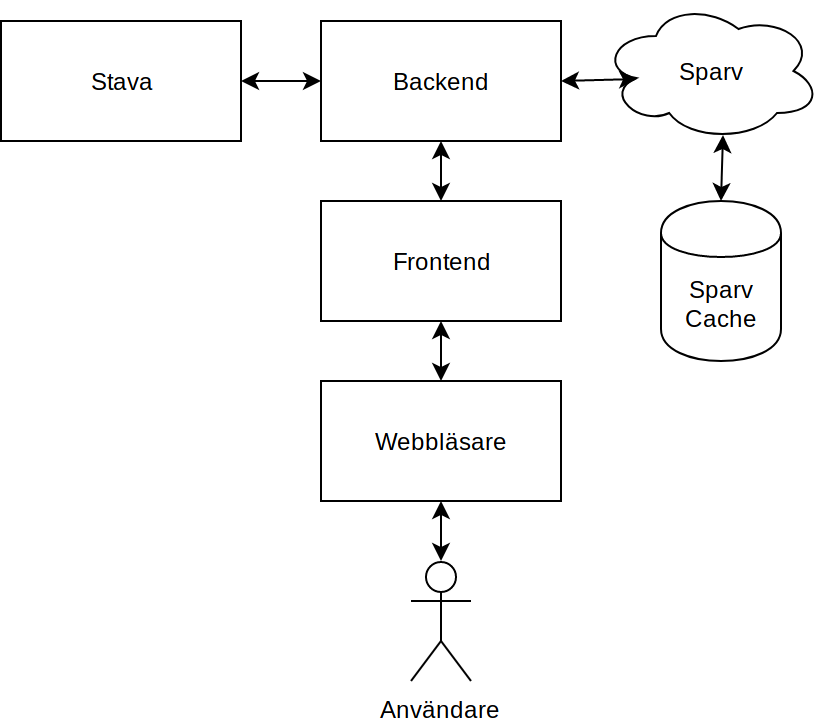
\includegraphics[width=0.75\textwidth]{architecture.png}
    \caption{Applikationens arkitektur}
    \label{fig:architecture}
\end{figure}

\subsubsection{Frontend}

Frontend utvecklades i markup språket Hyper Text Markup Language (HTML) för
strukturen och style sheet språket Cascading Style Sheets (CSS) ramverket
Bootstrap för en enhetlig design. Det är i frontend som användaren skickar in
sin rapport i docx-format och får tillbaka en analys av rapporten. Vi utvecklade
frontends användargränssnitt med integration i Canvas som mål och vi strävade
därför efter att så mycket som möjligt efterliknat Canvas grafiska gränssnitt
där man lämnar in uppgifter. Frontend är beroende av backend för att fungera
eftersom det är backend som har ansvar för att göra själva analyserna av
rapporterna. Frontend är därför bara ett gränssnitt som sköter kommunikationen
mellan backend och användaren.

\begin{figure}[H]
    \centering
    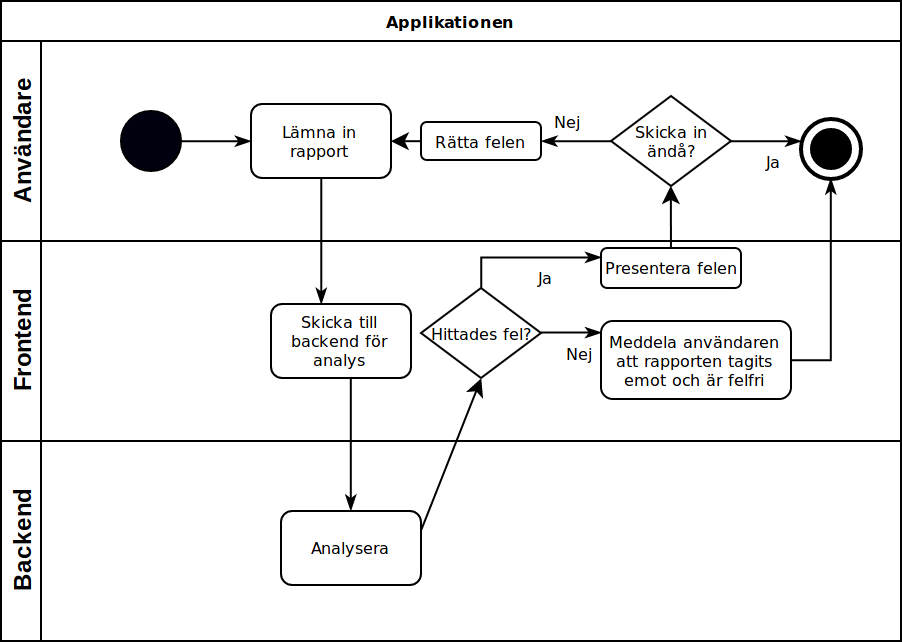
\includegraphics[width=0.95\textwidth]{overviewflow.png}
    \caption{Flödesdiagram som ger en överblick på hur man som student arbetar med applikationen}
    \label{fig:overviewflow}
\end{figure}

\subsubsection{Backend}

Backend utvecklades i Python och webbramverket Flask för att ta emot och skicka
data. Backend implementerar en webbAPI som kan ta emot rapporter i docx-format
och skicka tillbaka en analys av rapporten. Vi utvecklade backend
fristående så att den fungerar utan vår frontend eftersom vi ville att det
skulle vara så lätt som möjligt att integrera i andra system som inte är
intresserad av ett användargränssnitt utan enbart APIn för att analysera
rapporter.

När en rapport tas emot i backend konverteras dess innehåll till en stor
textsträng som vår dokument tolkare konverterar till Python objekt. Varje
rubrik, mening, ord och identifierade namnigenkänningskategorier blir objekt
vars egenskaper kommer från Sparvs textannotationer. Backend gör sedan en analys
på dessa objekt som undersöker ifall rapporten följer de regler som vi har
implementerat utifrån polisens dokumentation för rapportskrivning. De regler som
rapporten bryter mot skickas till rapportens avsändare i en lista som innehåller
felmeddelande, position och rättningsförslag för varje fel i rapporten. En
textrepresentation av rapporten skickas ihop med felmeddelanden så att eventuell
frontend eventuellt kan visa upp varje fels position i rapporten.

\begin{figure}[H]
    \centering
    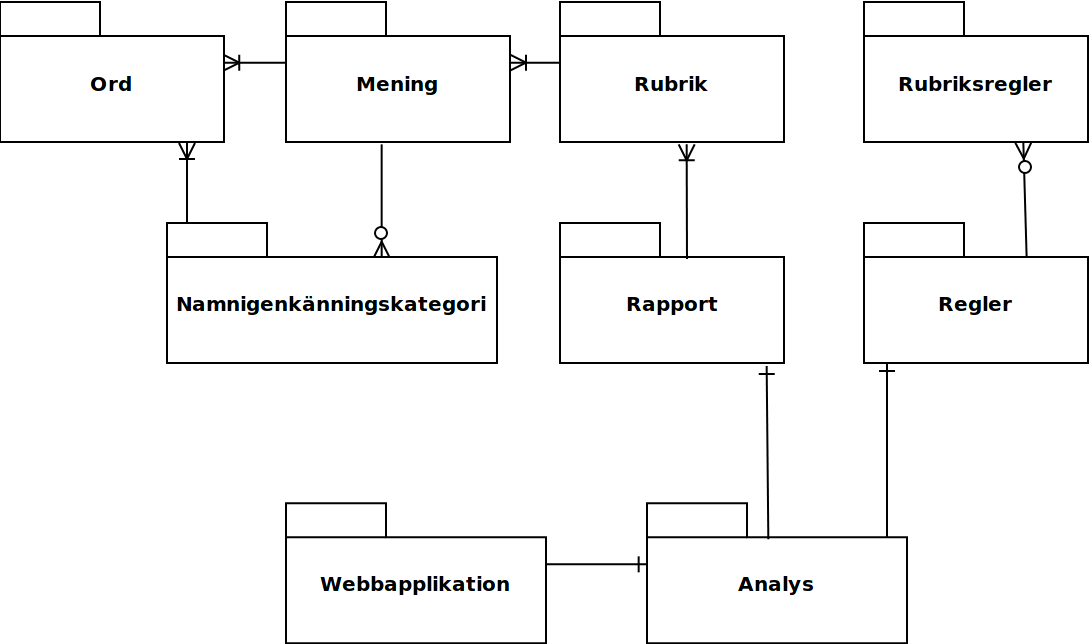
\includegraphics[width=0.75\textwidth]{backenderd}
    \caption{ERD diagram som visar klasser och dess relationer i backend}
    \label{fig:erdbackend}
\end{figure}

\subsubsection{Beroenden}

Applikationen använder en hel del externa verktyg för att göra analyser på
polisrapporterna. Anledningen till att vi här går igenom alla beroenden är inte
enbart för att den enskilde läsaren ska förstå hur applikationen fungerar utan
även för att göra det enklare för eventuella framtida utvecklare att
vidareutveckla applikationen. Följande rubriker beskriver vilka beroendena är
och varför vi använder dem. 
\\[1PC]
\textbf{Sparv} \newline
Sparv är ett verktyg som har utvecklats av Språkbanken vid Göteborgs universitet
för att annotera texter. Vår applikation konverterar rapporterna till ett
specialanpassat XML-format som den sedan skickar vidare till Sparv för
annotering. De typer av annotationer vi använder från Sparv i våra analyser är:

\begin{itemize}
\item \textbf{Grundform}: Ordens grundform, ex. \textit{Bananernas grundform är
    banan}
\item \textbf{Ordklass}: Ordens klass, ex. \textit{Kalle är ett egennamn och
    tjugotre är ett räkneord}
\item \textbf{Attitydvärde}: Ifall ett ord är positivt, negativt eller neutralt
\item \textbf{Namnigenkänning}: Kategoriserar textstycken i en grupp
  fördefinierade kategorier så som geografiska platser, föremål, tidpunkter och
  många fler
\item \textbf{Läsbarhetsindex (LIX)}: Ett mått som kan användas för att få en
  uppfattning om hur svår eller lätt en text är att läsa.
\end{itemize}
\textbf{Stava} \newline
Stava är ett stavningskontrollsprogram som är utvecklat av Viggo Kann och
Joachim Hollman på KTH. Anledningen till att vi valde att använda Stava för
stavningskontroll är att det är utvecklat för det svenska språket som många
stavningsprogram traditionellt sätt har svårt att hantera, \cite{kann:1997}
förklarar:

\begin{displayquote}
  Detta beror på att svenskan har många fler böjningsformer och framför allt att
  svenska ord kan vara sammansättningar som består av nästan hur många
  sammansättningsled som helst.
\end{displayquote}

Ett annat irriterande problem med rättstavningsprogram är att felstavningar av
vissa ord kan leda till att det blir ett nytt ord som är korrekt stavat men ändå
är fel i sammanhanget, dessa fel upptäcks inte av rättstavningsprogram som
enbart jämför ord mot ett lexikon. Stava har löst båda dessa problemen genom att
utföra en mosfologisk analys av texten och kan därmed tolka varje enskilt ords
betydelse i sammanhangen. Stava kommer med ett standardlexikon men tillåter
också att man lägger till egna lexikon vilket vi gjorde med ord som är speciella
för polisrapporter. När vi analyserar texter med Stava använder vi utöver
standardinställningarna några extra regler som gör att programmet känner igen
namn, förkortningar och ger rättningsförslag. Extra reglerna innebär att Stava
använder mycket mer datorkraft relativt mot att bara köra standardkontrollerna
men vi tog beslutat att det var värt det eftersom flaskpositiva och missade
stavfel minskar korrektheten och rättsäkerheten i rapporterna som lämnas in med
applikationen.
\\[1PC]
\textbf{Python beroenden}\newline
% [Lista varför och vilka Python bibliotek vi använder (de som har betydelse för analyserna)]

\subsubsection{Textanalys av rapporter}
% [Lista på de olika analyserna vi kör på rapporterna med referens till varifrån vi har tagit reglerna de bygger på]
% [Beskriv algoritmerna vi använder för att komma fram till resultat av analyserna..]
% [Användarguide som bilaga]

\begin{table}[H]
\centering
\begin{tabular}{|l|l|l|l|}
\hline
Regel                                & Lokalisering & Rättningsförslag & Referens \\ \hline
Felformatterade och saknade rubriker & Nej          & Ja               &          \\ \hline
Korrekt rubrik                       & Ja           & Ja               &          \\ \hline
Rubrikers beroende                   & Ja           & Ja               &          \\ \hline
Rubrikers ordning                    & Ja           & Ja               &          \\ \hline
Namnigenkänning                      & Ja           & Ja               &          \\ \hline
Läsbarhet                            & Nej          & Ja               &          \\ \hline
Känsliga ord                         & Ja           & Ja               &          \\ \hline
Oönskade ord                         & Ja           & Ja               &          \\ \hline
Polisförkortningar                   & Ja           & Ja               &          \\ \hline
Stavning                             & Ja           & Ja               &          \\ \hline
Grammatik                            & Ja           & Ja               &          \\ \hline
Tonalitet                            & Nej          & Ja               &          \\ \hline
\end{tabular}
\caption{Lista på reglerna vi har implementerat}
\label{rulestable}
\end{table}

\subsubsection{Verktyg och utvecklingsmiljö}

Båda applikationerna utvecklades i GNU Emacs 26.1 men det ska inte vara några
problem att använda andra utvecklingsmiljöer för att vidareutveckla
applikationen. Vi skrev i huvudsak applikationen i Python 3.7.3 med YAML som
konfigureringsspråk för backend samt HTML, CSS och Javascript för
användargränssnittet i frontend. För att vi skulle hålla reda på exakt version
av beroenden för applikationen använder vi Pipenv som är det officiellt
rekommenderade systemet för att hantera paket som applikationen är beroende av 
och virtuella miljöer förprogram skrivna i Python. Vi använde statisk typ 
kontroll i all Python kodeftersom kodbasen växte snabbt och blev uppdelad mellan 
många olika filer och då går det snabbare och är det lättare att förstå koden 
ifall metoder och variabler deklareras med typer.


\subsection{Resultat av användartester}

Användartesterna genomfördes den 9 april 2019 i ett grupprum vid Malmö
universitet. Fem personer deltog, varav fyra män och en kvinna, samtliga
studenter vid polisutbildningen i Malmö. Eftersom vi ville undvika risken att
deltagarna skulle påverkas av varandras åsikter valde vi att genomföra testerna
med en deltagare åt gången.

De placerades vid en bärbar dator, varpå applikationen samt en polisrapport
visades. Rapporten hade framtagits av oss utifrån det urval av studentmaterial
som Per Esbjörnsson bifogat, och texten var preparerad med ett tiotal vanliga
fel som vi observerat utifrån dessa. Felen inkluderade bland annat oriktiga
rubriker, nedsättande termer utan citationstecken och geografisk information som
utelämnats.

Efter en kort introduktion om projektet ombads deltagarna att ladda upp den
aktuella polisrapporten de hade framför sig till applikationen och sedan
korrigera texten utifrån de felmeddelanden som visades. Datorn var kopplad till
en tv-skärm som var belägen precis bakom deltagarna, detta för att vi som
testledare skulle kunna observera hur testet gick.

Vi försökte att ge så lite instruktioner som möjligt när deltagarna granskade
felmeddelandena och bidrog med förklaringar eller tips enbart när vi upplevde
att deltagarna blev alltför osäkra. Detta inträffade dock inte särskilt ofta.
När korrigeringarna gjorts ombads de att återigen ladda upp dokumentet. Testet
var därefter avslutat.

\subsubsection{SUS}

Efter testet fick deltagarna skriftligen fylla i SUS-formuläret. Vår uträkning
visade att det slutgiltiga värdet blev 83,5 poäng av 101 möjliga. Resultatet får
ses som ett gott omdöme då det är en god bit över det genomsnittliga värdet på
68, samt över 80 poäng vilket enligt \cite{laubheimer:2018} enbart tio procent av
webbsidor hamnar i.

\subsubsection{Intervju}

Vid den korta intervjun som följde därpå fick deltagarna besvara följande fem
frågor:
\begin{itemize}
\item Var felmeddelandena tydliga eller var det något specifikt du inte förstod?
\item Är det något i processen att lämna in en rapport som är oklart?
\item Finns det något du saknar med applikationen?
\item Tyckte du något var särskilt bra med applikationen, i så fall vad?
\item Tyckte du något var dåligt med applikationen, i så fall vad?
\end{itemize}

Två deltagare var samstämmiga i åsikten att en kortare genomgång av
applikationen behövdes innan de förstod processen men att den därefter var
tydlig för dem. En deltagare sa att denne särskilt tyckte om att de specifika
felen markerades i texten när felmeddelandet klickades på, en åsikt som också
bifölls av en annan deltagare med omdömet ”det gick väldigt snabbt att se vart
felen fanns i texten”. En tredje deltagare uttryckte att applikationen ”kan vara
ett jättestort hjälp till de som inte är bra på att skriva” samt att programmet
”kan vara bra på att hitta vanliga talspråksfel”. Fyra av fem deltagare
kommenterade att applikationen var tydlig som något särskilt bra.

\subsubsection{Önskvärda funktioner}

Två deltagare förde fram önskan att två eller flera intilliggande nedsättande
termer enbart skulle resultera i ett enda felmeddelande så att det blir tydligt
att dessa ska omgärdas av samma citattecken. Vår applikation avger också
felmeddelanden om gammeldags ord och uttryck, vilket en deltagare gärna hade
sett en motivering till varför sådana ska undvikas. Samma deltagare skulle också
vilja att felmeddelande visades i en kronologisk ordning utifrån vart i
dokumentet de återfanns, samt att olika färgkoder skulle kunna användas för att
gradera hur pass allvarliga de var. Personen såg även att vyn automatiskt
scrollade ner till det aktuella felet efter att deltagaren klickat på felet
utöver att bara markera dess plats i texten. Två deltagare hade velat kunna
kopiera text i felmeddelandena, och då i synnerhet när det fanns
rättningsförslag, för att effektivisera korrigeringsprocessen.

\section{Analys}

\section{Diskussion}

\section{Slutsatser och vidare forskning}


%
% Do not change
\newpage
\addcontentsline{toc}{section}{Referenser}

\bibliography{bibliography.bib}

\end{document}